\subsection{Land Use and Land Cover}\label{subsec:landuse}
\subsection*{Why You Need This Map}
The natural beauty of the Hudson Valley is a source of pride for its residents 
and is responsible for our strong tourism industry. Our challenge is to preserve 
the region’s remaining beauty while allowing for appropriate land uses that 
least impact the natural resources important to our health and the health of our 
biological communities.
\par
Smart land use decisions are more important than ever. Extreme weather events 
and drinking water pollution and availability have highlighted the effects of 
poor land use decisions. For example, the increase in impervious surfaces from 
development of structures, parking lots, and roads have made some communities 
more flood prone. The fragmentation of undeveloped areas by roads and 
development impedes wildlife movement and reduces habitat quality. Poorly 
placed developments, such as those sited too close to streams or on steeply 
sloped land, can result in declining stream health, degraded aquatic habitats, 
and lower water quality due to erosion and pollution. Even agricultural land 
uses can have detrimental effects in a watershed if poor management practices 
permit excess nutrients, sediment, and pathogens into waterways.
\par
Better land use decision-making must start with an understanding of our natural 
resources. By viewing land use and land cover data along with maps of streams, 
waterbodies, forest cover, wetlands and hydric soils, and other sensitive 
resources, communities can make better decisions for future growth. According to 
the Smart Growth Network, one of the principles of smart growth is to preserve 
open space, farmland, natural beauty, and critical environmental areas by 
directing new development to existing community centers. These rediscovered 
traditional planning principles from centuries past can reduce municipalities’ 
future infrastructure needs and costs, and foster more walkable communities that 
support commerce in community centers.
\par
Haeckel and Heady (2014) note that "land cover data sets\ldots should not be 
used for site planning and are not a viable substitute for on-the-ground 
knowledge and site visits\ldots" Satellite-derived land cover data do, however, 
allow planners, planning boards, elected officials, and developers to understand 
patterns of land use and to identify possible impacts of development proposals 
on the larger context of surrounding natural resources.

\subsection*{Orange County Context}
The National Oceanic Atmospheric Administration’s Coastal Change Analysis 
Program (C-CAP) Land Cover Atlas for Orange County reveals an increase in 
development and impervious surface area between 1996 and 2010: developed area 
increased by 14.23\% and impervious surface area 16.89\%. The majority of the 
increased development has been Low Intensity Developed (LID), which is 
typically comprised of single family housing, particularly in rural 
neighborhoods, but also includes all types of land uses. Forested and 
agricultural lands have lost the most land to development, with losses 
calculated at 6.06 square miles and 4.46 square miles, respectively. The chart 
below shows the percentages of total developed land and total impervious surface 
area in Orange County in 1996 and 2010.
\begin{table}[ht]
\begin{center}
    \begin{tabular}{| l | l | l |}
    \hline
    Land Cover Changes & 1996 & 2010 \\ \hline
    Percent Developed & 9.6\% & 10.97\% \\
    Percent Impervious Surface Area & 3.26\% & 3.81\% \\ \hline
    \end{tabular}
    \label{tab:lc_change}
    \caption{Land Cover Changes in Orange County between 1996 and 2010}
\end{center}
\end{table}

\subsection*{Land Cover Map}\
The Land Cover map shows natural land cover classes, such as forests and 
grasslands; semi-natural habitats, such as farmland, pastures, and managed 
woods; and developed land cover, which in the Town of Cornwall and the Village 
of Cornwall-on-Hudson can include residential, commercial, and institutional 
uses.
\par
The majority of land cover for the combined municipalities is forest (see 
Forests Map). Our communities are fortunate to be cradled by large, 
unfragmented forests in Storm King State Park and Black Rock Forest along the 
southeastern municipal boundary and in Schunnemunk State Park along the 
southwestern boundary. There is additional undeveloped land in the form of 
wetlands, cultivated cropland, and land planted for pasture/hay. Forested areas 
appear in shades of green.
\par
The map areas colored from pale pink to maroon represent the developed areas, 
with increasing percentages of imperviousness. Generally, the combined 
municipalities see development concentrations in the northeast areas in grid 
sections C2 and D2 as well as around Beaver Dam Lake straddling grid sections 
A1/A2 and B1/B2. Developed areas also follow the principal vehicular routes of 
Angola Road, Long Hill Road, Mineral Spring Road, Orrs Mill Road, Clove Road 
(aka County Road 27), State Route 94, State Route 32 (aka Woodbury Road), and 
Federal Highway 9W. The Village’s developed area is roughly a third of its total 
land cover. The Town’s developed area accounts for roughly one eighth of the 
total land cover.
\par
Cross referencing the Land Cover map with the Steep Slopes Map illustrates that 
development in the Town and Village is primarily located on slopes of less than 
15\%. Some development has occurred in the more wooded and steeper mountainous 
slopes between 15.1\% and 25\%. Future development on these slopes is 
discouraged due to the increased propensity for erosion and expensive drainage 
treatments that may not work for the long term. Additionally, building in the 
more mountainous areas results in loss of forest cover and wildlife habitat. 
Only in relatively few areas have the Town and the Village built on very steep 
slopes of greater than 25\%. Current zoning no longer allows for construction on 
very steep slopes.
\par
Agricultural production is present in Cornwall, represented on the map as 
cultivated crops, hay, and pasture and running along the central area of both 
municipalities. These areas appear as browns, greys, and yellows. Cornwall's 
agricultural areas are also some of the most scenically beautiful areas in our 
communities. 
\par
Woody and emergent herbaceous wetlands (slate blues) occur primarily in the 
lower elevations in the northern part of the Town and along waterways. They are 
not readily apparent on this map, but can be best identified when cross 
referencing the ~\nameref{map:wetlandsandhydricsoils}. More details on the distribution 
of wetlands in the municipalities are included in ~\nameref{subsec:wetland}.

\includepdf[pages=-,fitpaper]{cornwall_maps/LandCover.pdf}
~\label{map:landcover}
\subsection{Farmland}\label{subsec:farmland}
\subsection*{Why You Need This Map}
Agriculture is a significant part of the economy and character of the
communities in Orange County and New York State. The Hudson Valley in
particular has seen a boom in agro-tourism, breweries and distilleries, and
organic farming operations that feed urban demand for locally-sourced produce.
The definition of farmland in this chapter includes actively cultivated
cropland, livestock pastures, orchards, hayfields, and nurseries. Statewide,
there are more than 35,000 farms on approximately 7 million acres, which
represents more than 20\% of the state (NYS Agricultural Society). New York
ranks high among the major agricultural states in the nation, ranking in the
top 10\ in production of 30 commodities. It is the second largest producer of
apples, snap beans and maple syrup, third in cabbage, grapes and dairy, which
is largest segment of the State's agricultural sector, and fourth in pears (NYS
Dept. of Agriculture and Markets). Even so, farmland in New York is rapidly
diminishing in the face of increased residential development and the decline of
small family-owned farms. According to the American Farmland Trust:
\begin{itemize}
    \item More than 4,000 farms in New York State have been lost to real estate
    development since the 1980s.
    \item More than 80\% of the fruits and vegetables grown in New York come 
    from farms that are currently threatened by development
    \item 30\% of New York farmland is owned by farmers who are over the age of 
    65
    \item Only 5\% of farmland in New York has been permanently protected
\end{itemize}
Creating an inventory of these farm parcels is vital to prioritizing the most 
important agricultural areas in the Hudson Valley region for preservation, and 
encouraging new agricultural commerce on existing farmland.

Soil quality and characteristics are the foundation of the agricultural economy 
in New York, and soil features like nutrient load, acid/pH balance, the ability 
to hold or drain moisture, slope, and texture (grain size), are all important 
for agricultural productivity. These characteristics differ widely based on 
things like the underlying geology, glacial history and flooding frequency, and 
soils can sometimes be very different even in two fields that are in close 
proximity. Because of the importance of these soil qualities, soils are very 
specifically classified by the U.S. Department of Agriculture. The 
classifications are then grouped into larger designations that generally 
indicate how productive the soil could be for agriculture. The chapters on 
~\nameref{subsec:calcareous} and ~\nameref{subsec:bedrock} provide additional 
detail on this topic and these designations.
%Calcareous and Glacial Outwash Soil

\subsection*{Farmland Soils and Agricultural Parcels in the Town of Cornwall 
and the Village of Cornwall-on-Hudson}
If agriculture is important to the regional economy and the character of the 
Town, then it is important to know where farms are, and the location of soils 
that best lend themselves to farming. This map shows where various farm parcels 
are located within Cornwall’s borders, as well as where the best agricultural 
soils are located, as identified by the U.S. Department of Agriculture. 

Cornwall does not have an abundance of farm parcels. Much of what was once 
farmland has been developed for residential, commercial and municipal uses over 
the centuries. The majority of remaining farmland parcels are located in the 
western part of the town and are dedicated to field crops like hay and horse 
farming pastures. There are a number of vacant farm parcels that feature 
prominently on the Meadows, Grasslands, and Shrublands Map. Also visible on the 
map, are a single parcel classified as orchard located at Jones Farm, and a 
single parcel classified as livestock and products along Route 94. 

The shaded areas showing Prime Farmland, Prime Farmland If Drained, and Soils 
of Statewide Importance match the areas profiled on the General Soil Classes 
map. More detailed descriptions of these soils can be found in the General Soil 
Classes chapter and the glossary for this \gls{nri}.

\includepdf[pages=-,fitpaper]{cornwall_maps/FarmlandSoilsandAgParcels.pdf}\label{map:farmlandsoilsandagparcels}
\subsection{Conservation and Public Lands}\label{subsec:conservation}
\subsection*{Why You Need This Map}
Conservation and public lands are areas where the natural resources identified 
in this report are most likely to be protected from future development. By 
mapping our existing protected lands, we can see where we can be confident that 
these natural resources are secure. Perhaps more importantly, we can find the 
gaps where there are important natural resources that are not yet protected, 
and identify areas that should be prioritized by the community for future 
protection. Of particular importance are undeveloped areas that act as linkage 
zones between existing preserved lands. Linking and expanding these natural 
habitats can help sustain healthy wildlife populations and reduce the potential 
for isolated habitat islands that are created when natural areas become 
surrounded by development. 
\par
Our region is fortunate in that there are several large blocks of protected 
land including Storm King State Park, Black Rock Forest Preserve, and 
Schunnemunk Mountain State Park. Each of these protected areas consists of over 
1,500 acres that are rich in natural resources that will never be threatened by 
development. Much of this land was protected through the work of state agencies 
and non-profit organizations with a mission to conserve natural resources. There 
are numerous non-profit organizations that are active in the area, including 
Black Rock Forest Consortium, Hudson Highlands Land Trust, Open Space 
Institute, Orange County Land Trust, and Scenic Hudson, and the amount of 
protected land is likely to continue to grow through their work. 
\par
The categories of protected land shown on the maps included with this report 
have differing methods and levels of protection. Conservation easements are 
areas where the land is owned privately, but future development is restricted in 
order to protect the property’s conservation values. Municipal Parks may be 
protected with a primary goal of providing recreational opportunities to the 
community. There are also properties that are not shown on the map that are not 
formally protected, but function as conservation lands because they are owned by 
an entity that values natural resources such as an educational institution. 

\subsection*{Protected Open Space Map}\label{subsec:protectedopenspace}
The Town of Cornwall and Village of Cornwall-on-Hudson have significant areas of 
protected land. Together, these municipalities contain 7,473 acres1 of protected 
land, which represents approximately 38\% of the land in these municipalities. 
Approximately 21\% of the Village of Cornwall-on-Hudson is protected. 

The following is a description of the categories of protected land within the 
Town of Cornwall and Village of Cornwall-on-Hudson.

\paragraph{State Parks: 2,933 Acres}Storm King State Park and Schunnemunk State Park are partially located in the Town of Cornwall. These parks are managed by the Palisades Interstate Park Commission, and they are open to the public for passive recreation.

\paragraph{Nature Preserves: 2,024 Acres}
Black Rock Forest is the most significant protected area in the Town. Black 
Rock Forest consists of 3,643 acres, the majority of which are in Cornwall. The 
forest contains over 23 miles of trails that are open to the public for passive 
recreation. Black Rock Forest is also permanently protected by a conservation 
easement. 

Other nature preserves include the Leone Preserve, which is owned by the Orange 
County Land Trust, and the Hudson Highlands Nature Museum, which is also 
permanently protected by a conservation easement.

\paragraph{Conservation Easements: 987 acres}
There are 10 conservation easements in the Town and Village, which are held by 
various non-profits, including the Hudson Highlands Land Trust, Open Space 
Institute, Orange County Land Trust, and Scenic Hudson. 

\paragraph{Municipal Parks: 79 acres}
Municipal parks include Riverlight Park, Roe Park, and Harold Avenue Park 
(Laurel Crest Park) in the Town, and Donahue Memorial Park in the Village. Some 
of these parks are designed and developed for active recreation with ball 
fields and facilities (such as Riverlight Park), while others are largely 
undeveloped and open for passive recreation (such as Roe Park).

\includepdf[pages=-,fitpaper]{cornwall_maps/ProtectedOpenSpace.pdf}\label{map:protectedopenspace}
\subsection{Zoning and Tax Maps}\label{subsec:zoning}
\subsection*{Why You Need These Maps}
New York State's zoning enabling statutes state that comprehensive plans must 
provide for the "immediate and long-range protection, enhancement, growth, and 
development" of a locality, with land use regulations, including zoning, 
"conform[ing] to the locality's comprehensive plan" (Salomone 2004).1 All land 
use regulations are enacted to "promote the public health, safety, and general 
welfare;" "[z]oning is primarily enacted to control the use of land and the 
density of those uses"~\citep{haeckel2014}.  Local zoning can also impose 
greater restrictions than state law to protect, for example, natural areas and 
cultural resources, such as historic locales, scenic areas, groundwater, 
floodplains, wetlands, and wildlife habitats.

The following maps for the Town of Cornwall and Village of Cornwall-on-Hudson 
show the zoning districts, special overlays/districts, and tax parcels within 
our community. The narrative will focus primarily on considerations for 
additional protective measures for our natural resources as authorized by 
Municipal Home Rule Law (Salomone 2004). The natural resources found in each 
district are described in relationship to the permitted uses within each 
district in Appendix F – Natural Resources within Zoning Districts and Overlays 
for the Town of Cornwall and the Village of Cornwall-on-Hudson.

\subsection*{Zoning and Parcels}
The following sections will focus on recommendations for additional measures 
important to the immediate and long-range protection of our quality of life and 
natural resources. Some recommended protective measures are applicable to both 
the Town and Village. (Additional information regarding the recommended 
measures below can be found in Appendices C, H, I, and J.)2

\subsubsection{Town of Cornwall}
Zoning Chapter 158 of the Code of the Town of Cornwall describes the uses 
allowed in 12 zoning districts and 2 overlays. The tables of General Use 
Regulations provide an overview of the uses permitted by right, uses by special 
permit, and permitted accessory uses.
\begin{itemize}
    \item The Town should consider developing an aquifer protection overlay 
    district as well as a Source Water Protection Plan to protect the supply 
    and quality of drinking water.  Exclusion of bulk storage should be 
    considered.
    \item The Town should consider developing steep slope regulations that limit 
    construction on slopes exceeding 15\% to protect against erosion, 
    sedimentation of streams and down-slope areas, landslides, and the 
    degradation of scenic views.
    \item The Town should consider strengthening current language pertaining 
    to tree removal (see chapter 75 – Clearing and Grading) by developing tree 
    preservation legislation. Such legislation would enable the Town and its 
    residents to take advantage of the natural benefits that are intrinsic to 
    trees: 
    flooding control, filtration of pollutants and prevention of erosion, 
    protection of watershed areas, improvement of air quality, noise barriers, 
    habitat for wildlife, and cooler micro-climates.
    \item The Town’s zoning chapter 90, Freshwater Wetlands Protection Law, is 
    very comprehensive. The Town should consider improving the Law by supporting 
    the identification of wetlands as small as half an acre and applying the 
    existing Law to this wetland size.3 (Half an acre of wetland can store up 
    to three-quarters million gallons of floodwater at no cost to a 
    municipality.) The identification of smaller wetlands can be done as a 
    citizen science project in partnership with the Cornwall Conservation 
    Advisory Council, the Cornwall Central School District, and community 
    residents.4 Additionally, the Town should explore providing adequate 
    protection for inter-jurisdictional wetlands by working to develop equally 
    protective regulations with adjoining municipalities.
    \item Throughout the Town’s Code, the presence of a wetland can result in 
    the denial of a permit for clearing and grading and/or building within a 
    100-foot buffer. However, no such language exists for streams. The Town 
    should consider developing a Stream Buffer Overlay for perennial and 
    seasonal waterways in order to maintain water quality, recharging of 
    groundwater, waterway health for wildlife, and bank stabilization and 
    erosion control. A minimum buffer of 200 feet is recommended; wider buffers 
    should be considered for habitat protection of specific wildlife (see 
    Strong, 2008). Orange County has developed a model riparian buffer local 
    law.
    \item The Town’s Code includes language referencing the minimization of 
    public and private losses from flood conditions by controlling the 
    alteration of natural floodplains and their associated stream channels 
    and natural protective barriers.  The Town should consider developing a 
    Floodplain Overlay District to clearly outline areas to be protected 
    and, given the increase in severe storms, also consider protections to 
    the five-hundred-year floodplain.
    \item The Town should consider referencing green infrastructure practices 
    as part of Code Chapter 121 on Stormwater Management.
    \item The Town should consider expanding the application of Conservation 
    Subdivision Design Layout to all districts currently zoned MCR and ARR as 
    well as increasing the minimum percentage of open space to 80\%. The 
    positive resulting impact from these changes would include less expensive 
    construction costs, less clearing and grading, and preservation of the 
    visual and environmental integrity of most of the landscape (OCWA 2014).
    \item The Town should consider tasking the Cornwall Conservation Advisory 
    Council with the development of a comprehensive listing of native plantings 
    to support the intent of the Ridge Preservation Overlay District. 
    Additionally, a listing of said planting can be made available to 
    developers, residents, and businesses to further enhance the beauty of our 
    Town without inviting nuisance plant species. (See Village recommendation 
    for additional detail.)
\end{itemize}

\includepdf[pages=-,fitpaper]{cornwall_maps/TownZoning.pdf}\namedlabel{map:townzoning}{Zoning and Parcels Map}
\subsubsection{Village of Cornwall-on-Hudson}
Zoning Chapter 172 of the Code of the Village of Cornwall-on-Hudson describes 
the uses allowed in 6 zoning districts and 2 overlays.
\begin{itemize}
    \item The Village should consider managing stormwater by limiting 
    impervious coverage through maximum development coverage areas rather than 
    maximum lot coverage percentages. The former limits the portion of a lot 
    covered by buildings, parking areas, accessory structures, and other 
    impervious materials.
    \item The Conservation Residential CR-3 District (scenic) provides for a 
    conservation green belt setback of 25 feet along both sides of Deer Hill 
    Road where no tree cutting, construction, or other development is 
    permitted. The Village should consider adding language to encourage 
    bringing properties into conformance.
    \item The Village should consider incorporating language that encourages the 
    use of native plantings suitable for hardiness zone 6. NYSDEC’s Division of 
    Lands and Forests provides many native suggestions for flowers; grasses, 
    ferns, groundcovers; shrubs; trees; and vines.
    \item The Industrial District’s currently permitted uses may be negatively 
    impacted by projected sea level rise. The Village should consider 
    additional limitations on industrial uses or additional precautionary 
    measures of currently permitted uses that may negatively impact the 
    aquifer, wetlands, and floodplains present.
    \item The Village should consider referencing green infrastructure 
    practices as part of Code Chapter 132 on Stormwater Management and for 
    off-street parking for 10 or more vehicles.
    \item The Village should consider developing a Floodplain Overlay District 
    to clearly outline areas to be protected and, given the increase in severe 
    storms, also consider protections to the five-hundred-year floodplain.
    \item The Village should consider developing a Wetlands and Watercourses 
    Overlay with a minimum buffer of 200 feet for surface waters of the State of 
    New York.
    \item The Village should consider a minor amendment to Chapter 151 Trees, 
    Shrubs, and Bushes to increase successful plantings of trees on private 
    properties: burlap should be removed prior to planting.
\end{itemize}
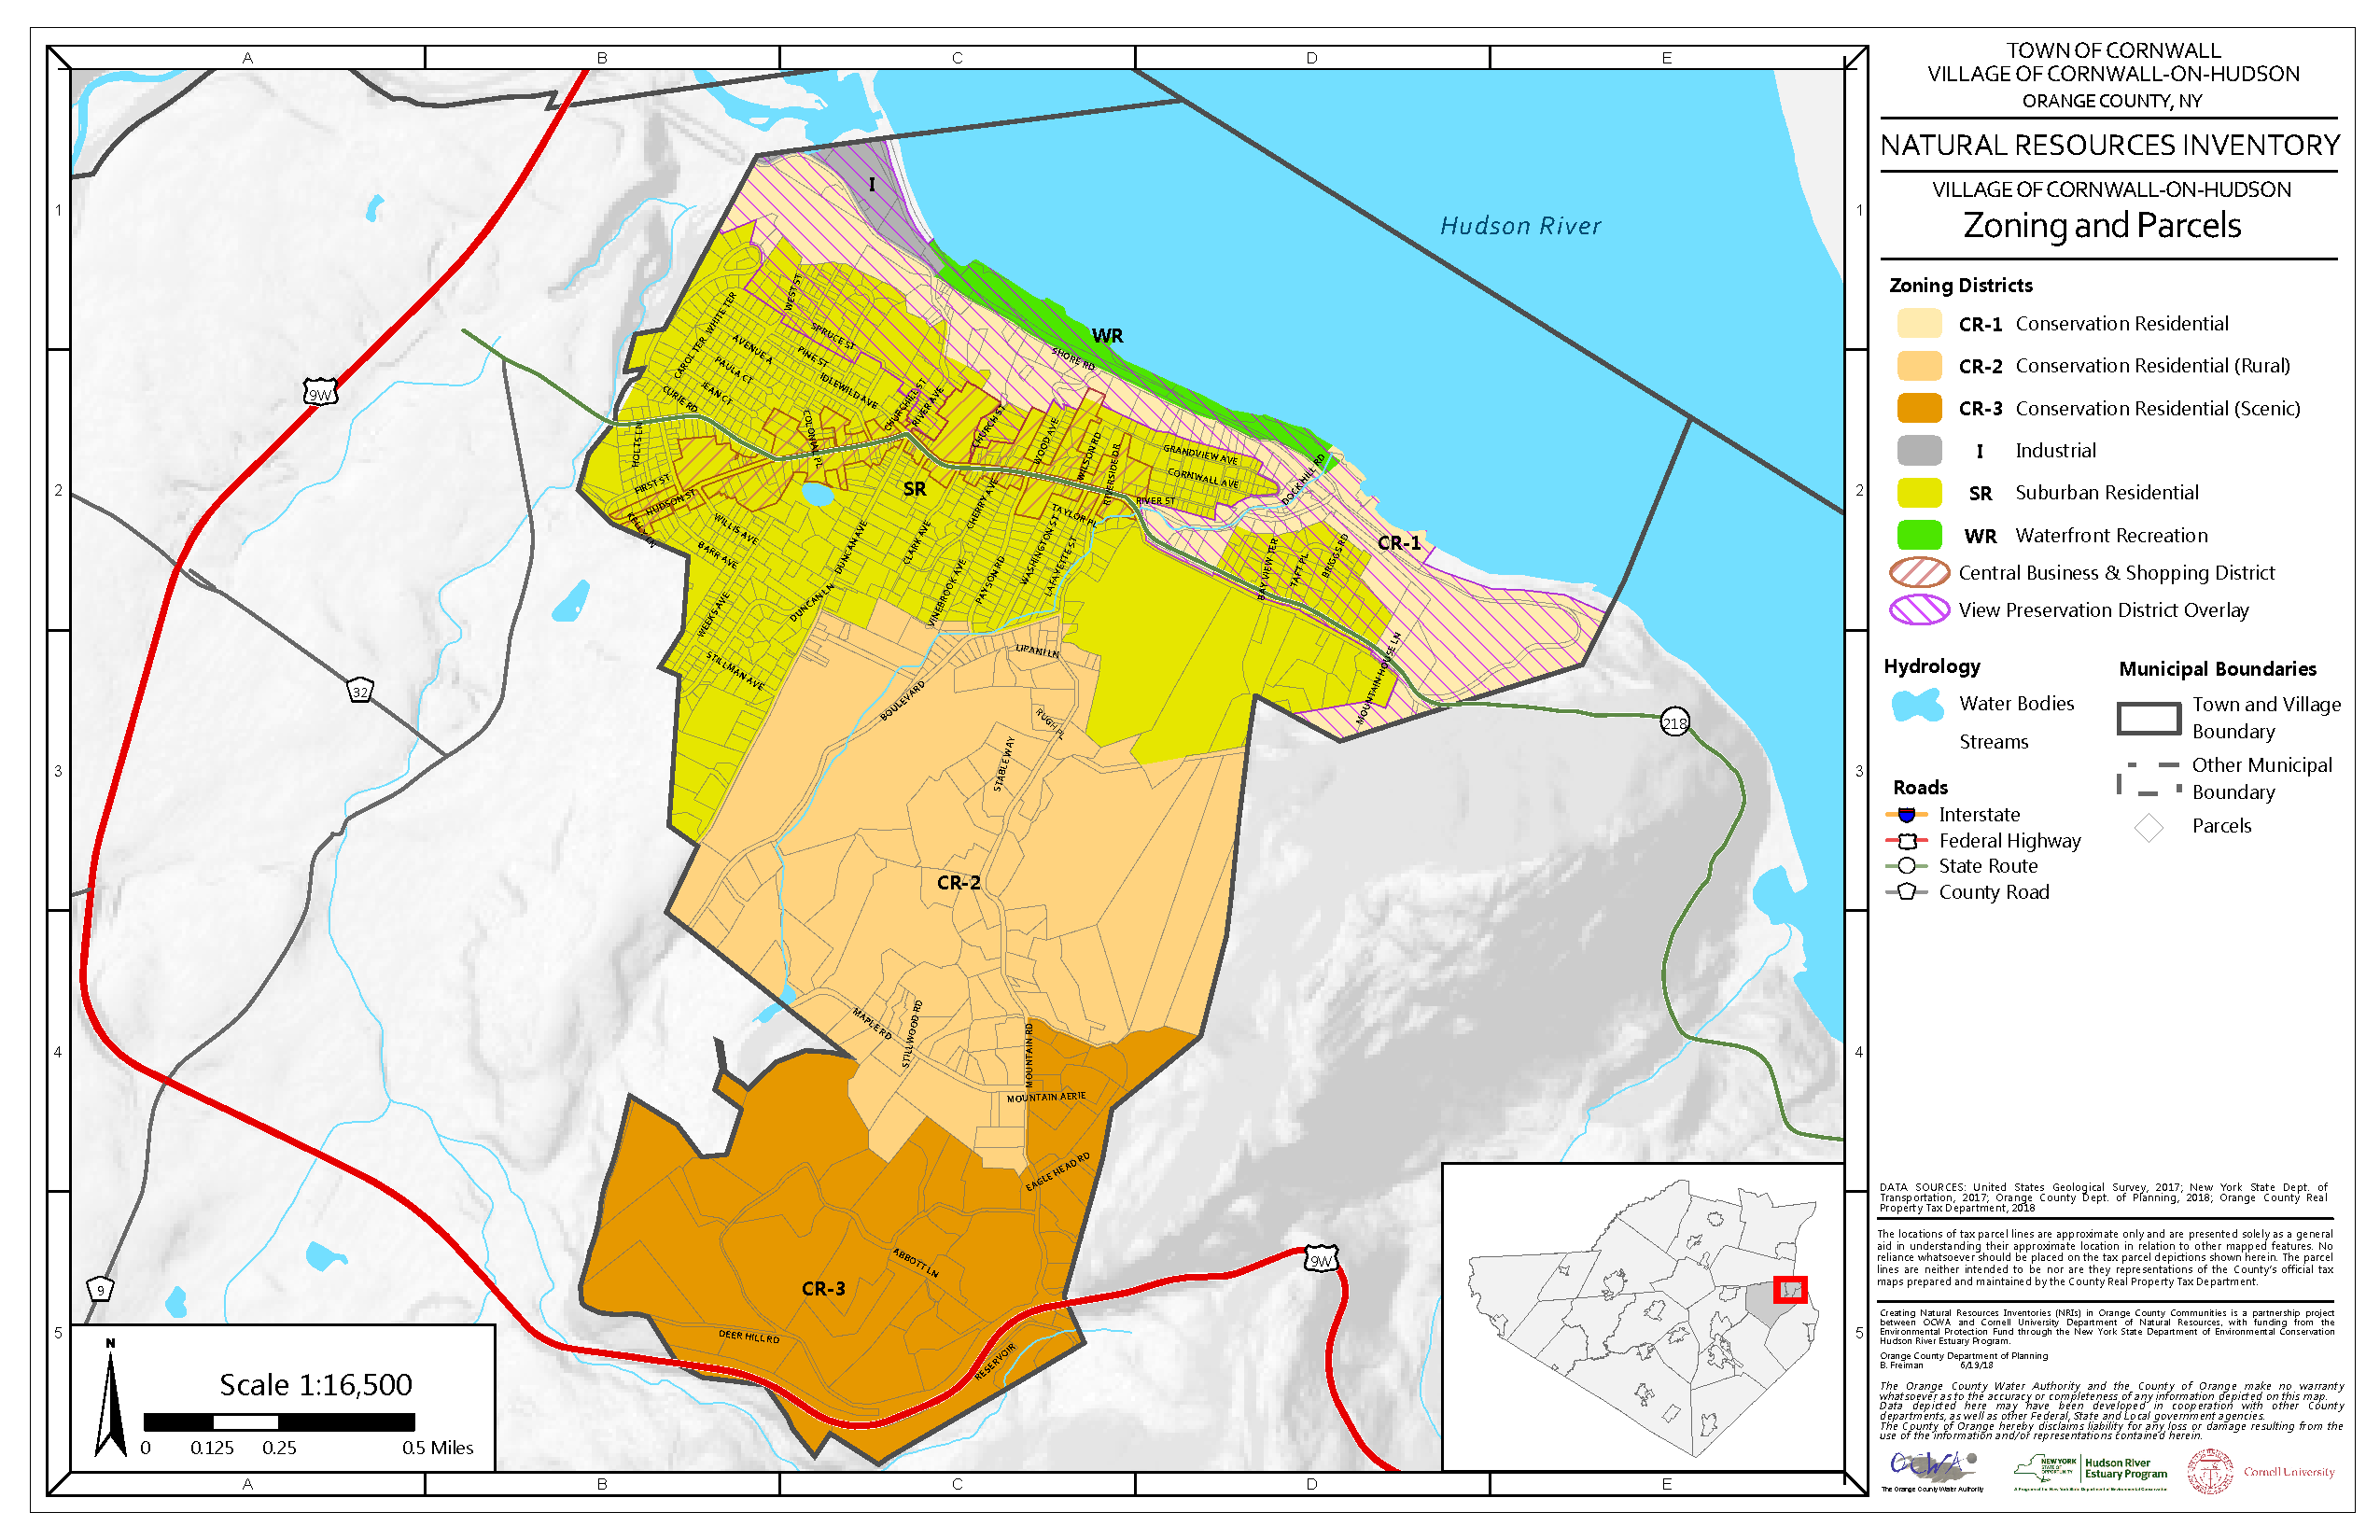
\includepdf[pages=-,fitpaper]{cornwall_maps/VillageZoning.pdf}\label{map:villagezoning}